\documentclass[12pt]{article}
\usepackage[english]{babel}
\usepackage{natbib}
\usepackage{url}
\usepackage[utf8x]{inputenc}
\usepackage{amsmath}
\usepackage{graphicx}
\graphicspath{{images/}}
\usepackage{parskip}
\usepackage{fancyhdr}
\usepackage{vmargin}
\setmarginsrb{2.5 cm}{1 cm}{1 cm}{2.5 cm}{1 cm}{1.5 cm}{1 cm}{1.5 cm}


\usepackage{float}

\title{Preparation of Tritium Spiked Water}								% Title
%\author{}								% Author
%\date{}											% Date

\makeatletter
\let\thetitle\@title


%\pagestyle{fancy}
%\fancyhf{}
%\rhead{\theauthor}
%\lhead{\thetitle}
%\cfoot{\thepage}

\begin{document}

%%%%%%%%%%%%%%%%%%%%%%%%%%%%%%%%%%%%%%%%%%%%%%%%%%%%%%%%%%%%%%%%%%%%%%%%%%%%%%%%%%%%%%%%%

\begin{titlepage}
	\centering
    \vspace*{0.5 cm}
	\rule{\linewidth}{0.2 mm} \\[0.4 cm]
	{ \huge \bfseries \thetitle}\\
	\rule{\linewidth}{0.2 mm} \\[1.5 cm]
	
\end{titlepage}

%%%%%%%%%%%%%%%%%%%%%%%%%%%%%%%%%%%%%%%%%%%%%%%%%%%%%%%%%%%%%%%%%%%%%%%%%%%%%%%%%%%%%%%%%



%%%%%%%%%%%%%%%%%%%%%%%%%%%%%%%%%%%%%%%%%%%%%%%%%%%%%%%%%%%%%%%%%%%%%%%%%%%%%%%%%%%%%%%%%

\section{Acquire a clean Container}
Ensure that the container is clean, sterilized and dry.
\subsection{Weigh the empty container}
\begin{figure}[H]
    \centering
    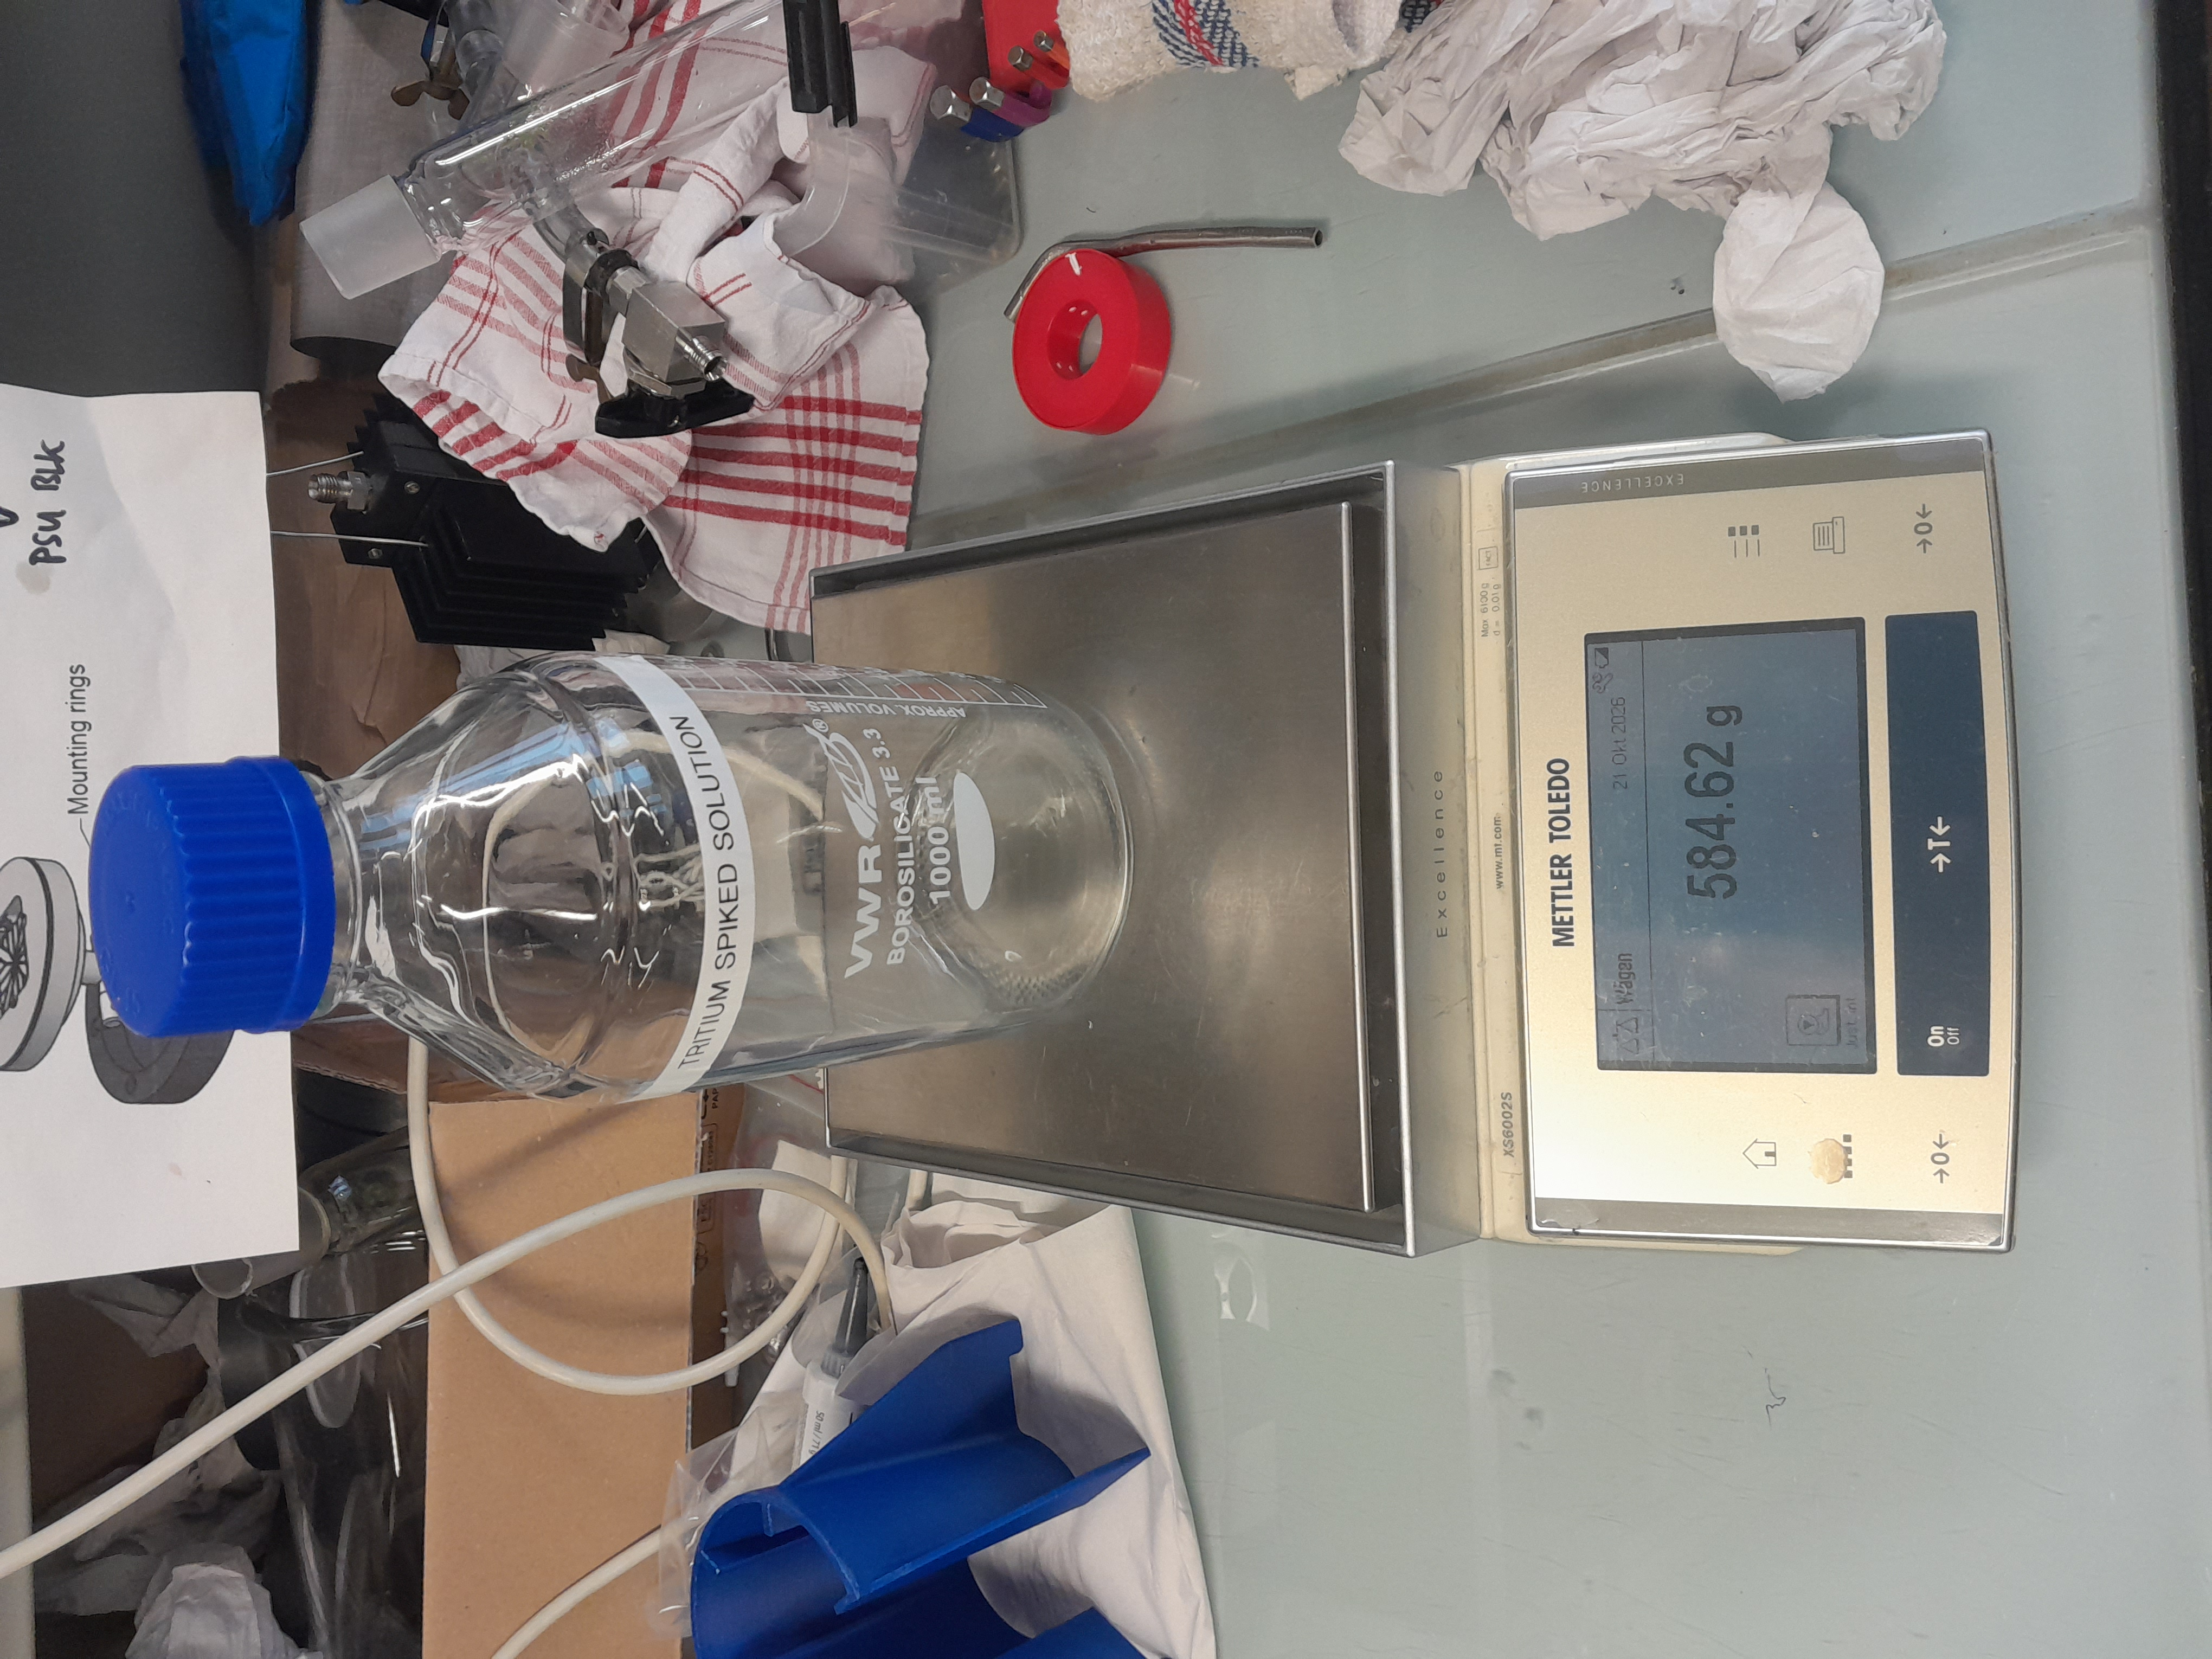
\includegraphics[width=0.5\linewidth,angle=270]{20261021_105423.jpg}
    \caption{Weighing of the clean empty container}
    \label{fig:1}
\end{figure}
For example the mass of the bottle as displayed in the figure m\textsubscript{b}= 584.62 g.
\subsection{Add tritium free water}
Tare the balance and add a target amount of tritium free water to the bottle and weigh it.
\begin{figure}[H]
    \centering
    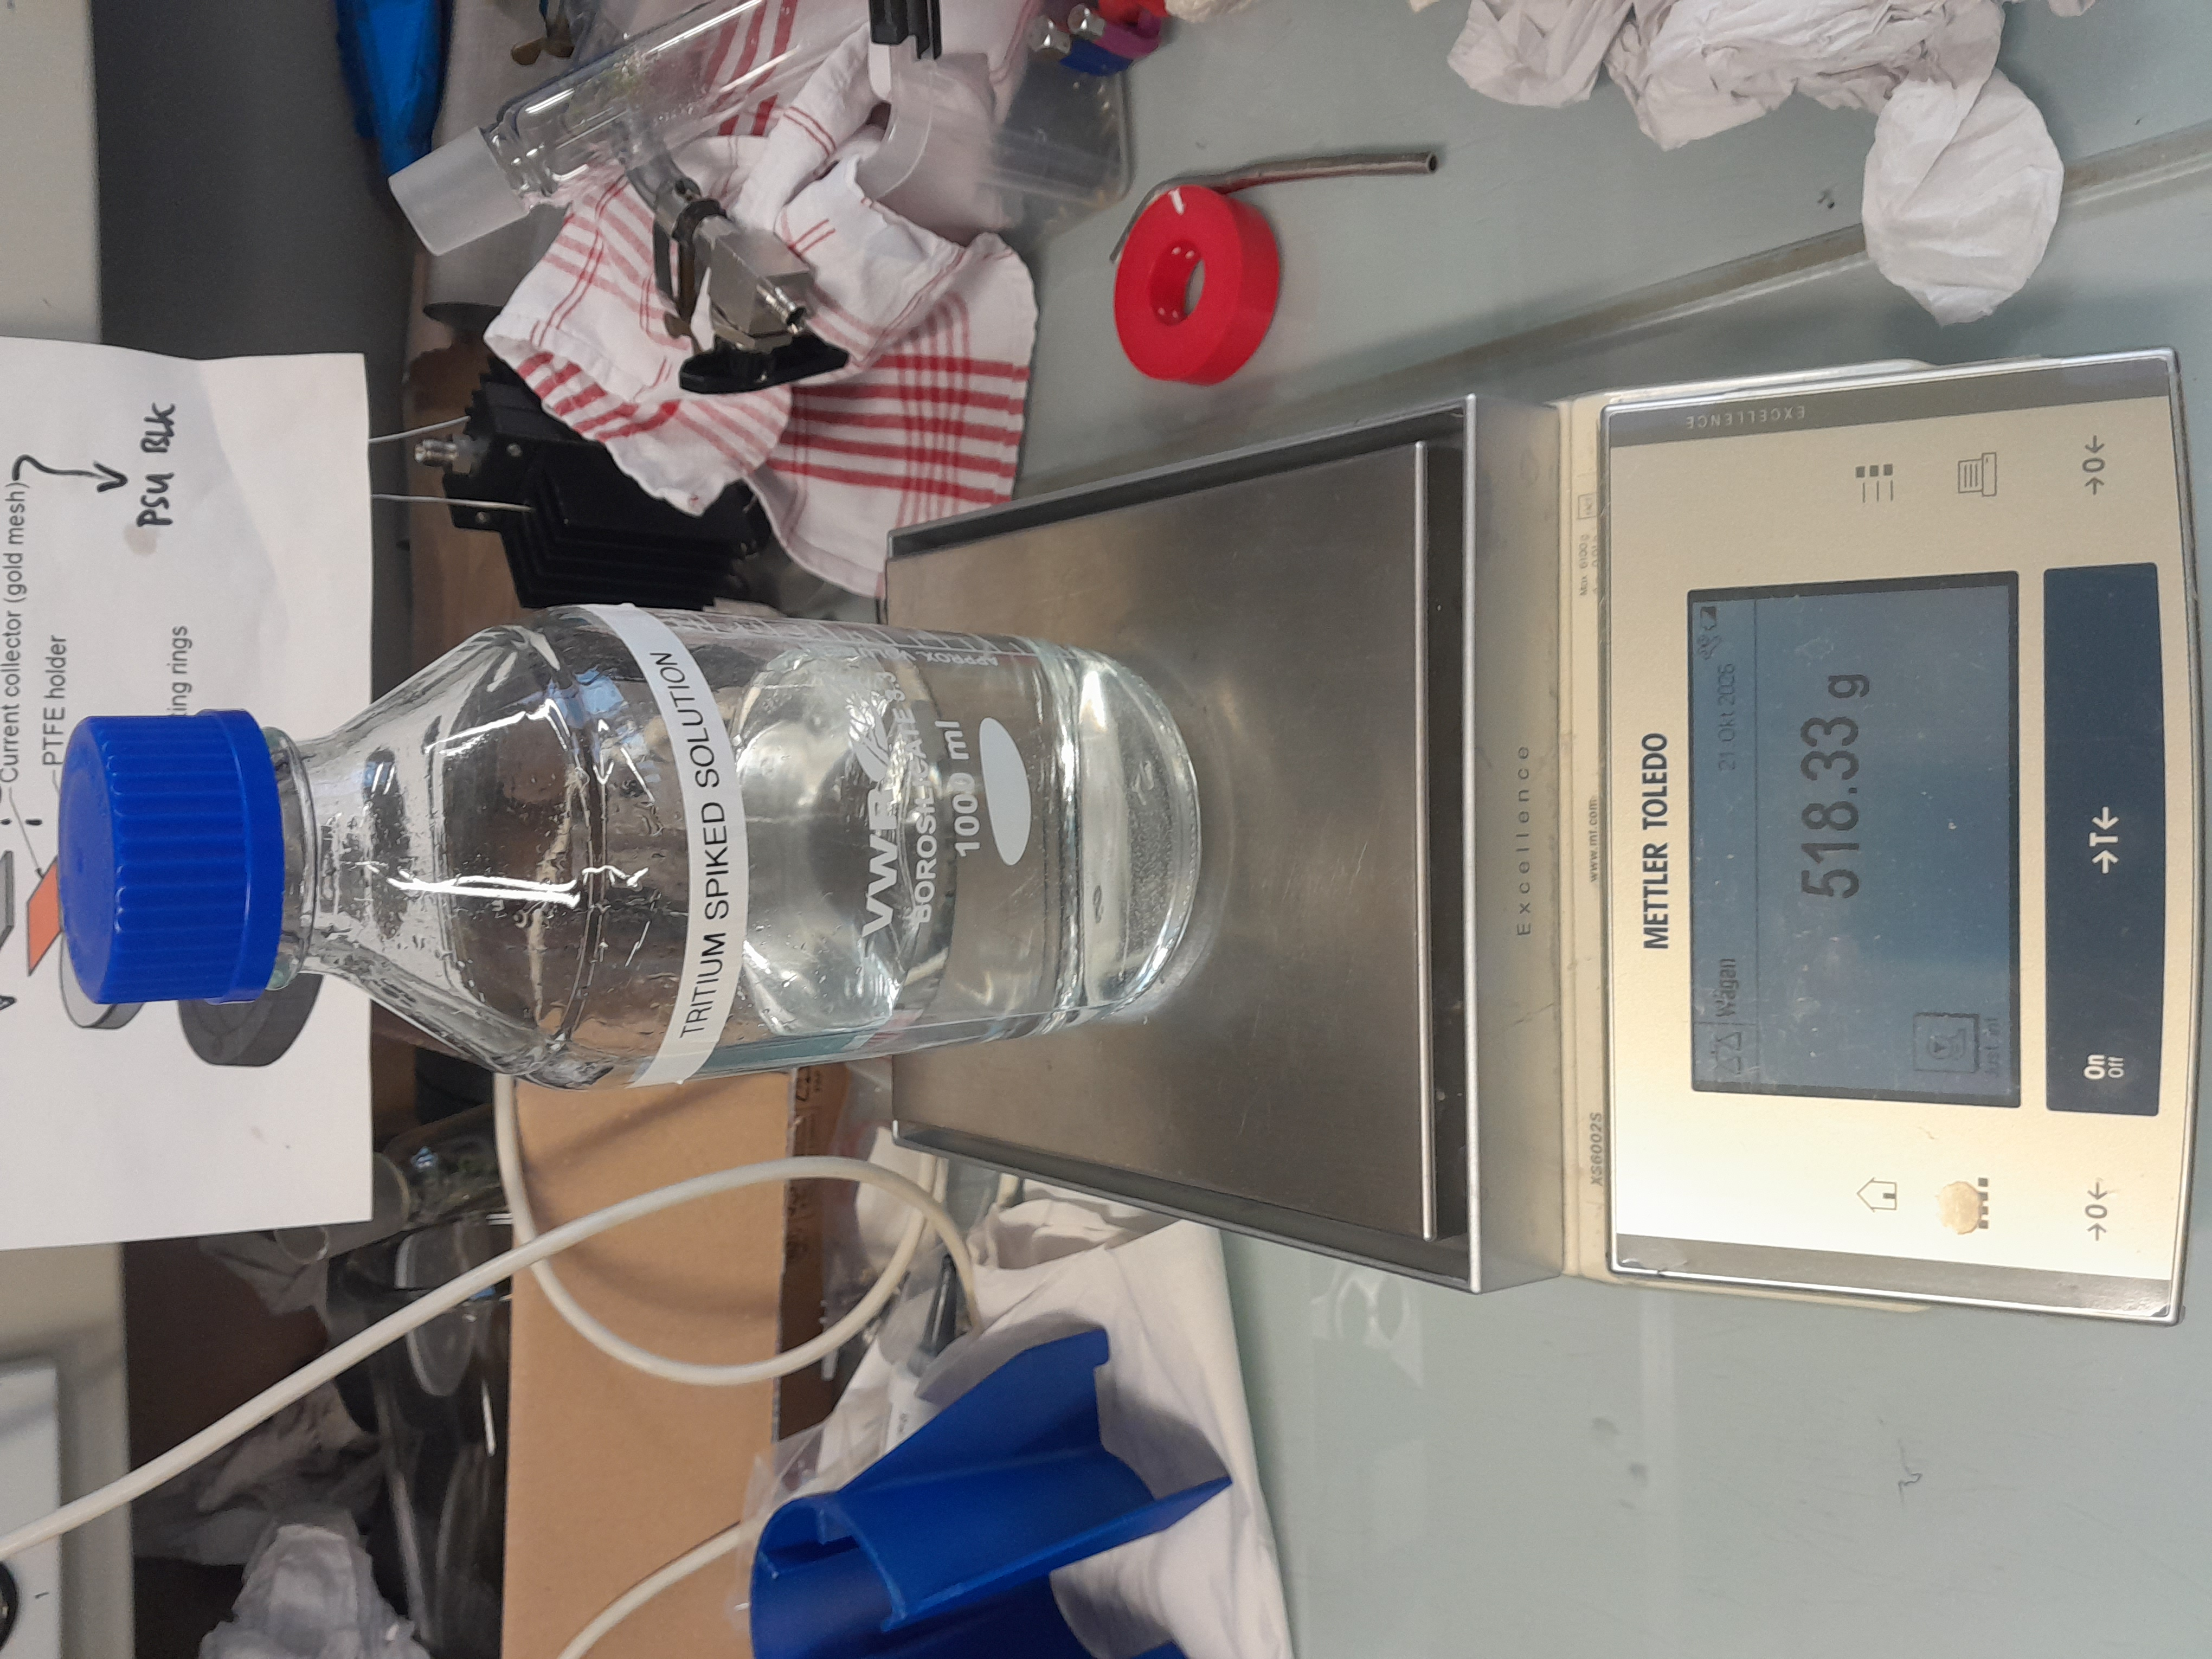
\includegraphics[width=0.5\linewidth,angle=270]{20261021_105816.jpg}
    \caption{Weighing of tritium free water}
    \label{fig:2}
\end{figure}
For example the mass of tritium free water as displayed in the figure m\textsubscript{tfw}= 518.33 g
\subsection{Add the tritium standard}
Tare the balance and add a target amount of the tritium standard to the bottle and weigh it.
\begin{figure}[H]
    \centering
    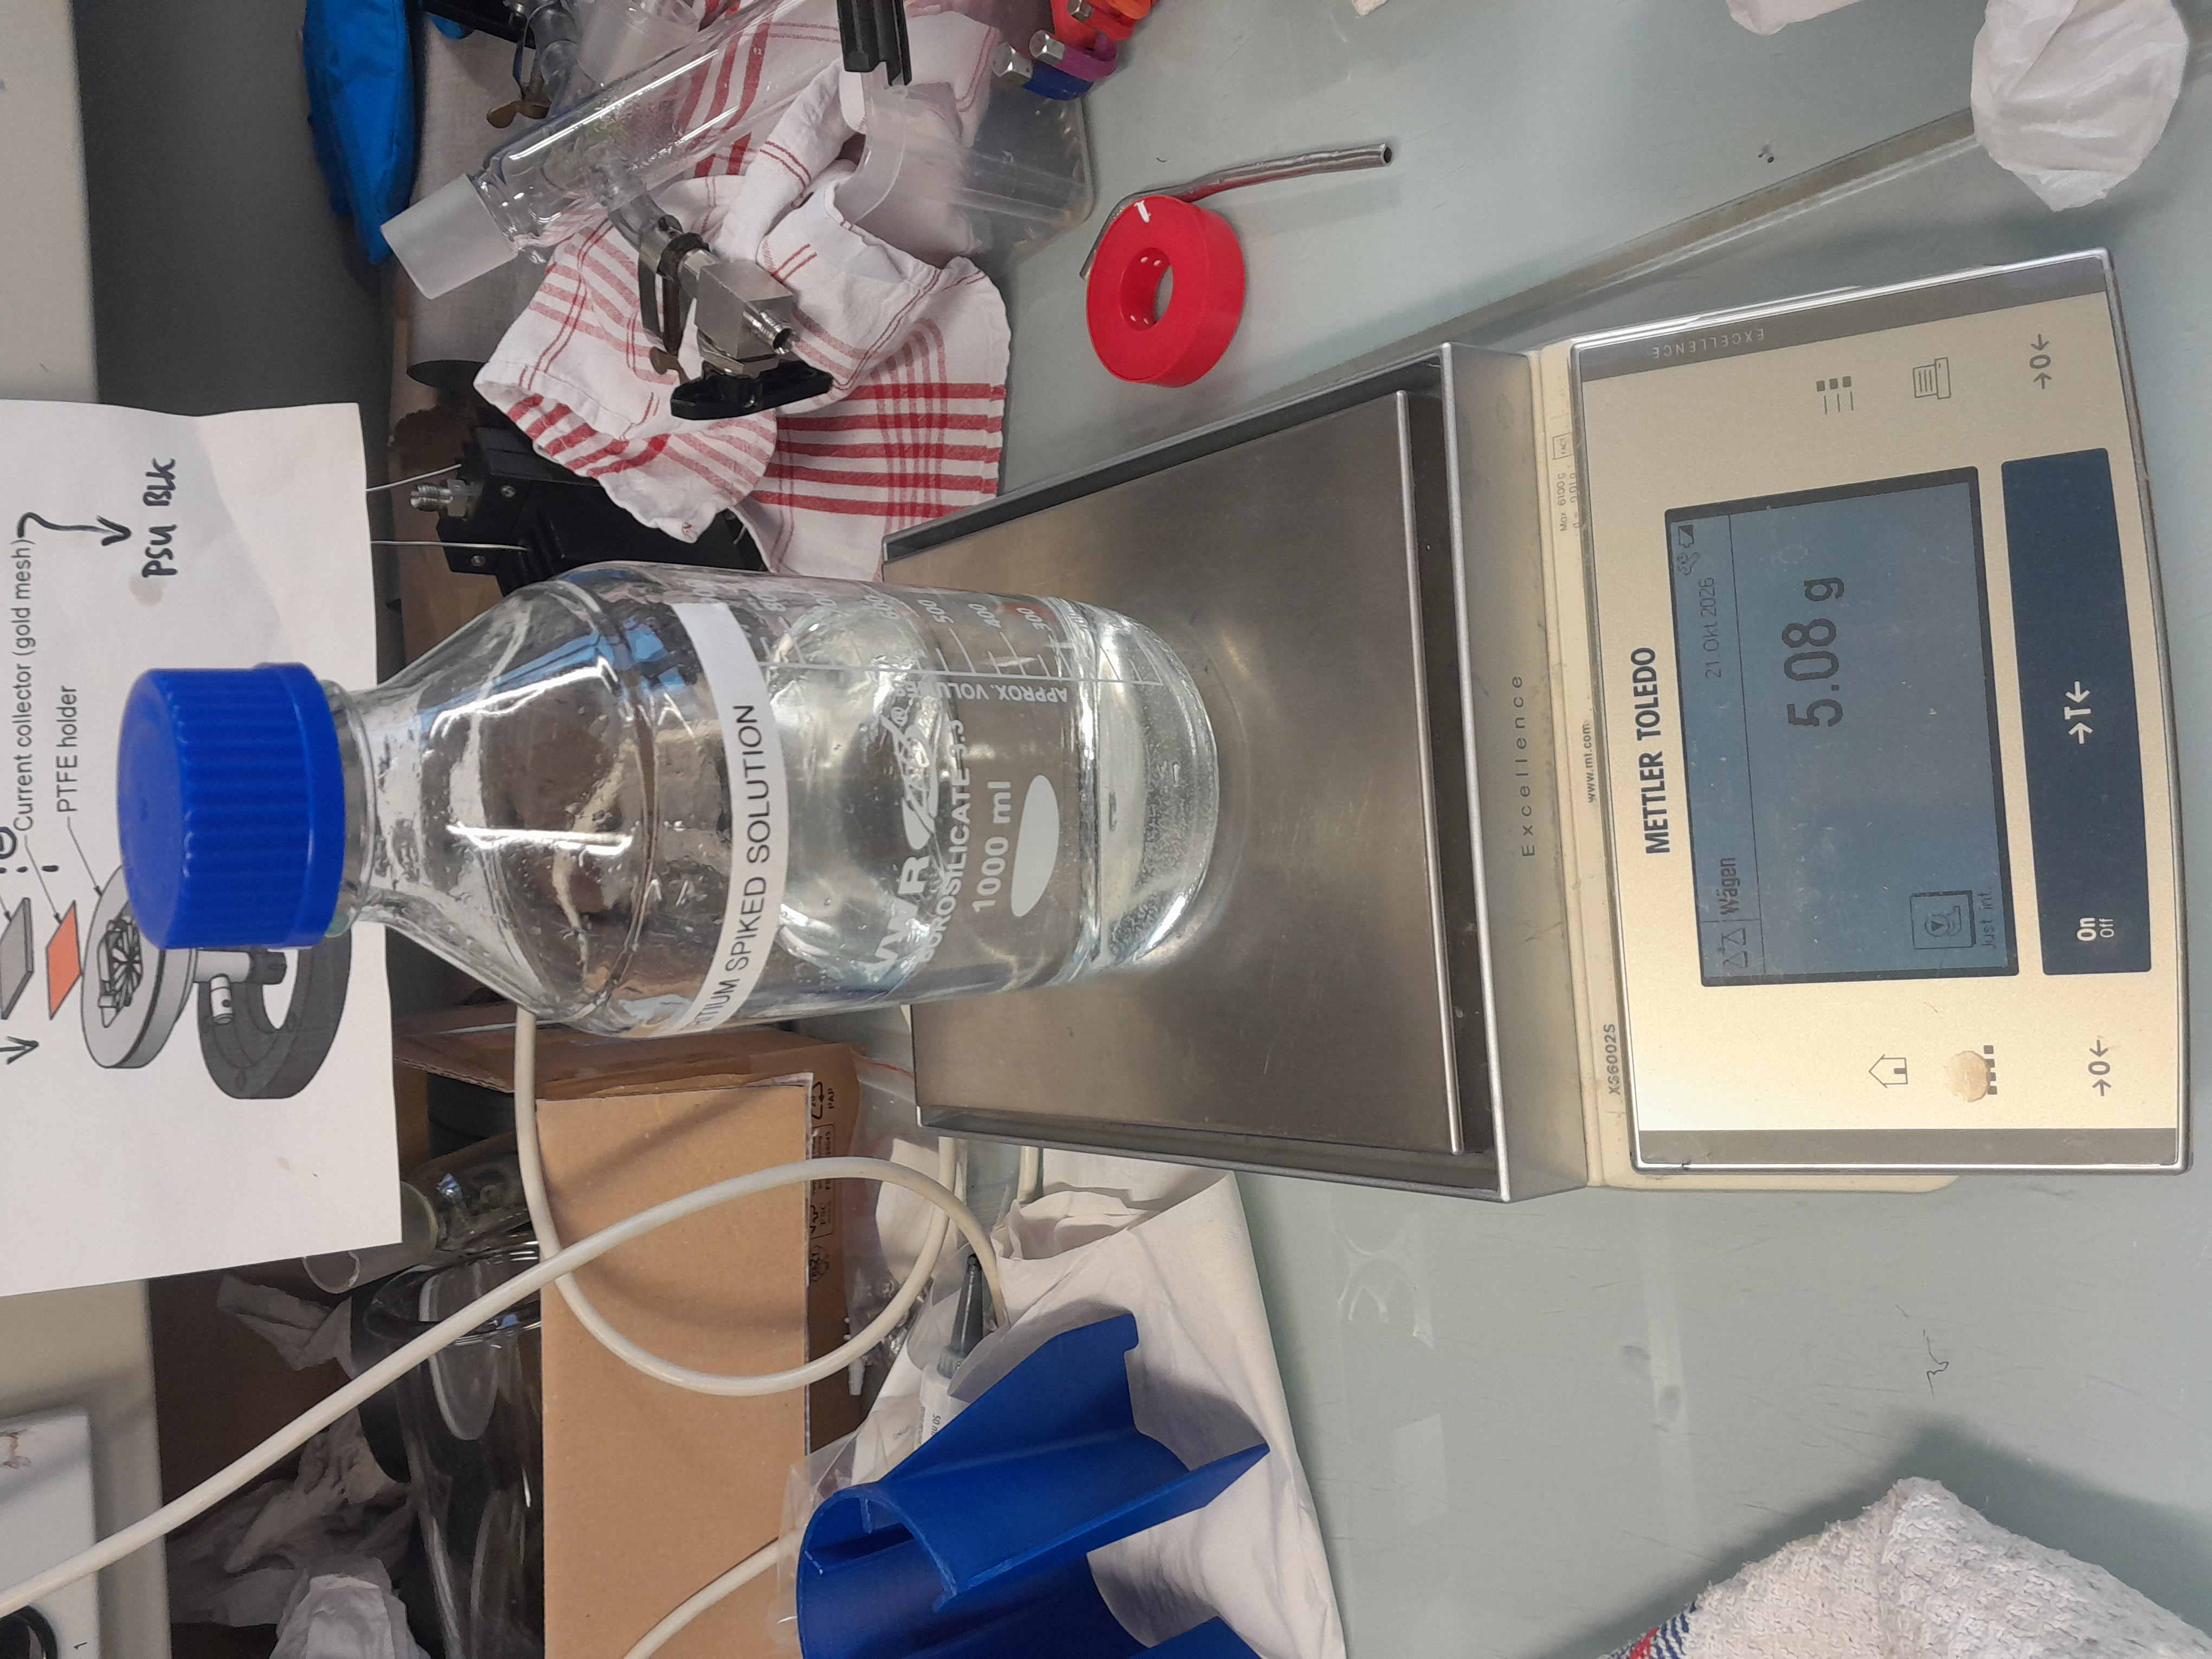
\includegraphics[width=0.5\linewidth,angle=270]{20261021_110333.jpg}
    \caption{Weighing of tritium standard}
    \label{fig:3}
\end{figure}
For example the mass of tritium standard as displayed in the figure m\textsubscript{s}= 5.08 g

\subsection{Compute the final activity}
\begin{itemize}

\item Use the decay equation to determine the current activity of the standard.
\begin{equation}
T(t)=T_0
\left(\frac{1}{2}\right)^{t/t_{1/2}},
\end{equation}
take t\textsubscript{1/2}= 4500 days
\item Use the concentration relation to determine the final activity of the spiked solution
\begin{equation}
T_f=\frac{T_{s}m_{s}}{m_{s}+m_{tfw}}
\end{equation}
where T\textsubscript{f} is the final activity and T\textsubscript{s} is the activity of the standard spiked solution, T\textsubscript{s} is the current activity of the standard, m\textsubscript{s} is the mass of the standard and m\textsubscript{tfw} is the mass of tritium free water.

\item The 15046 TU (REF 24.10.2018) standard was used. Therefore as of 21/10/2026 the activity of the spiked solution in figure \ref{fig:3} is 93.15 TU.
\end{itemize}
%\newpage
%\bibliographystyle{plain}
%\bibliography{biblist}

\end{document}